\subsection{Motivation}
\begin{frame}
\frametitle{Introduction}
\begin{columns}
    \column[t]{4.5cm}
	\begin{figure}[htbp!]
		\begin{center}
			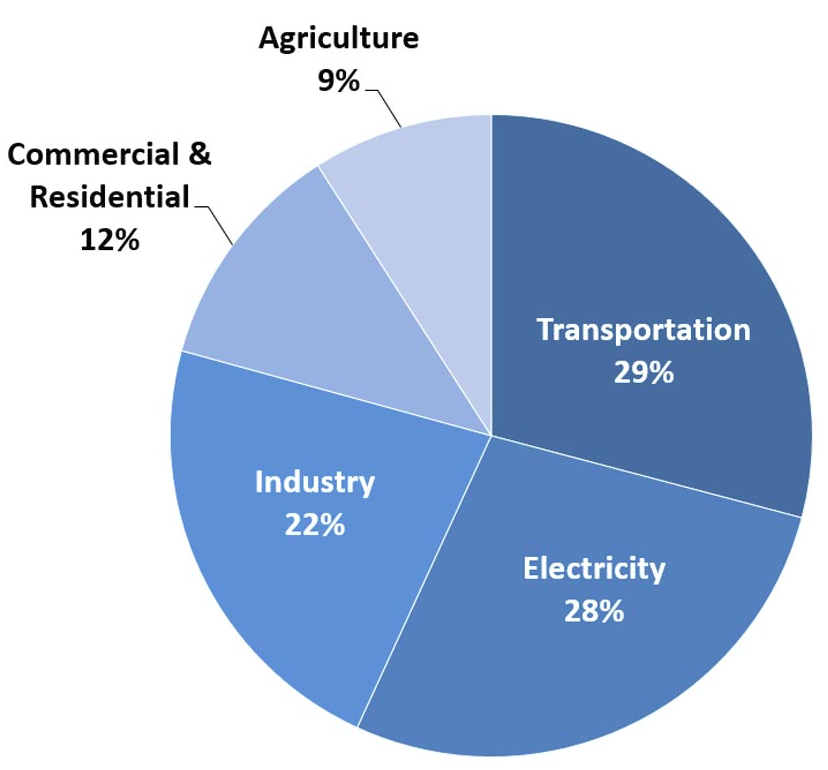
\includegraphics[height=4.5cm]{images/total-ghg-2017.png}
		\end{center}
		\caption{Total U.S. GHG Emissions by Economic Sector in 2017. Image reproduced from \cite{us_epa_sources_2020}.}
	\end{figure}

	\column[t]{5.5cm}
	\\
	Illinois Climate Action Plan (iCAP) \cite{isee_illinois_2015}:
	\begin{itemize}
		\item American College and University Presidents’ Climate Commitment.
		\item Main goal: carbon neutrality by 2050.
	\end{itemize}
	\vspace{0.5cm}
	Six target areas:
	\begin{itemize}
		\item Energy conservation.
		\item Energy generation, purchasing, and distribution.
		\item Transportation.
		\item Water and storm water.
		\item Waste and recycling.
		\item Agriculture, land use, and food.
	\end{itemize}
\end{columns}
\end{frame}

% Notes:
% Transportation and Electricity are the economic sectors that produced ...

\subsection{Finding a solution}
\begin{frame}
\frametitle{Transportation}
\begin{columns}
	\column[t]{4.cm}
	\\
    Fuel Cell Electric Vehicles (FCEV):
	\begin{itemize}
		\item Address global warming concerns.
		\item Limitation on fossil fuel supply.
		\item Examples:
		\begin{itemize}
			\item Japan: Fuel cell vehicles, trucks, buses, forklifts.
			\item California: 1000 refueling stations by 2030.
			\item Champaign-Urbana: Expects 2 Hydrogen buses in 2020.
		\end{itemize}
	\end{itemize}

    \column[t]{6.cm}
	\begin{figure}[htbp!]
		\begin{center}
			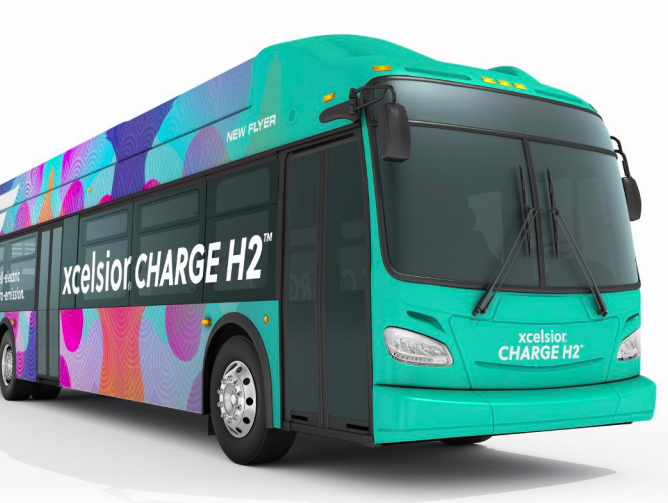
\includegraphics[height=5cm]{images/bus.png}
		\end{center}
		\caption{New Flyer fuel cell bus. Image reproduced from \cite{new_flyer_xcelsior_2020}.}
	\end{figure}
\end{columns}
\end{frame}


\begin{frame}
\frametitle{Energy generation}
\begin{columns}
	\column[t]{4cm}
	\\
	Obvious solution:
	\begin{itemize}
		\item More renewables.
	\end{itemize}

    New problem:
	\begin{itemize}
		\item Duck curve.
		\item Net demand ramps.
		\item Over-generation.
	\end{itemize}

    Consequences:
	\begin{itemize}
		\item Increase in dispatchable generation.
		\item Decrease in non-dispatchable generation.
	\end{itemize}

    \column[t]{8cm}
	\begin{figure}[htbp!]
		\begin{center}
			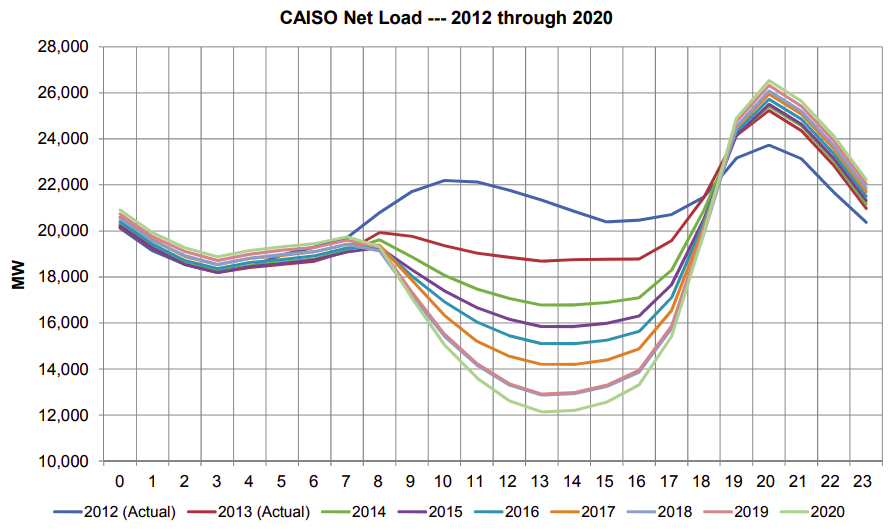
\includegraphics[height=4.7cm]{images/caiso-duck.png}
		\end{center}
		\caption{The duck curve. Image reproduced from \cite{bouillon_prepared_2014}.}
	\end{figure}
\end{columns}
\end{frame}


\begin{frame}
\frametitle{A possible solution}
    \textbf{Nuclear reactors and hydrogen:}
    \begin{itemize}
    	\item DOE and INL established the Next Generation Nuclear Plant (NGNP) \cite{us_nrc_next_2017}.
		\item Office of Nuclear Energy (NE): H2@Scale initiative \cite{office_of_nuclear_energy_could_2018}.
		\item Energy produced with no carbon emissions.
		\item Produce hydrogen as main/secondary product.
		\item Hydrogen as fuel for the FCEV.
		\item Hydrogen as electricity storage.
	\end{itemize}

	\centering
	\vspace{0.7cm}
	\textbf{Approach consistent with our goal of reducing carbon emissions!!}
\end{frame}


\begin{frame}
\frametitle{Microreactors}
\begin{columns}
	\column[t]{5cm}
	\begin{itemize}
		\item Several designs are under development in the US.
		\item Plug-and-play reactors.
		\item Remote commercial applications.
		\item Remote military bases.
	\end{itemize}
	\vspace{0.6cm}
	Features:
	\begin{itemize}
		\item Factory fabricated.
		\item Transportable.
		\item Self-regulating.
	\end{itemize}

    \column[t]{6cm}
	\begin{figure}[htbp!]
		\begin{center}
			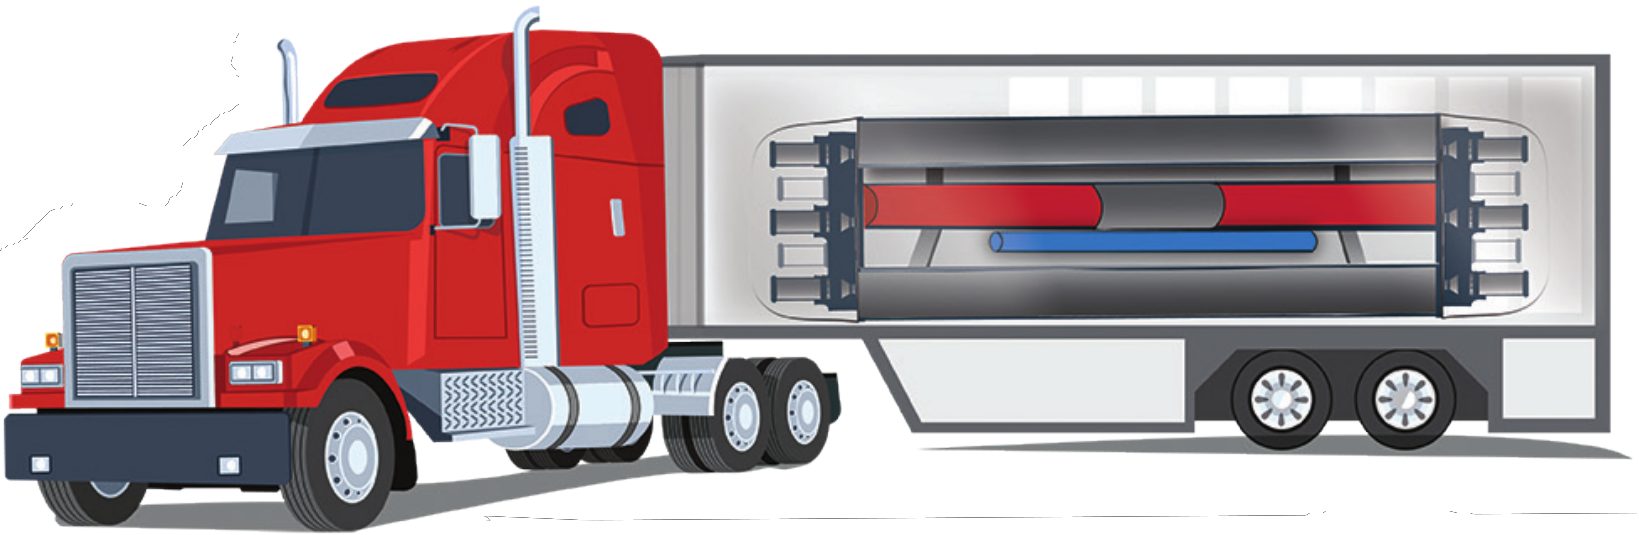
\includegraphics[width=5.8cm]{images/microreactor}
		\end{center}
		\caption{Microreactor design. Image reproduced from \cite{us-doe_ultimate_2019}.}
	\end{figure}
\end{columns}
\end{frame}

\subsection{Objectives}
\begin{frame}
\frametitle{Objectives}
\centering
    \begin{enumerate}
    	\item Replace use of fossil fuels by CU MTD and UIUC fleets with hydrogen.
    	\item Supply the hydrogen with one or many microreactors.
    	\item Analyze the magnitude of the duck curve in UIUC grid.
        \item Mitigate the negative effects of the duck curve.
	\end{enumerate}
\end{frame}